
% v2-acmsmall-sample.tex, dated March 6 2012
% This is a sample file for ACM small trim journals
%
% Compilation using 'acmsmall.cls' - version 1.3 (March 2012), Aptara Inc.
% (c) 2010 Association for Computing Machinery (ACM)
%
% Questions/Suggestions/Feedback should be addressed to => "acmtexsupport@aptaracorp.com".
% Users can also go through the FAQs available on the journal's submission webpage.
%
% Steps to compile: latex, bibtex, latex latex
%
% For tracking purposes => this is v1.3 - March 2012
\documentclass[prodmode,acmtecs]{acmsmall} % Aptara syntax
\usepackage[spanish,polish]{babel}
\usepackage[T1]{fontenc}
\usepackage{fancyvrb}
\usepackage{graphicx,hyperref}
\newcommand\cutout[1]{}


\usepackage[table]{xcolor}
\usepackage[utf8]{inputenc}
\usepackage[parfill]{parskip}
\usepackage{tabulary}
\PassOptionsToPackage{hyphens}{url}
\usepackage{hyperref}    
\usepackage[capitalize]{cleveref}


% Metadata Information
% !!! TODO: SET THESE VALUES !!!
\acmVolume{0}
\acmNumber{0}
\acmArticle{CFP}
\acmYear{0}
\acmMonth{0}

\newcounter{colstart}
\setcounter{page}{4}

\RecustomVerbatimCommand{\VerbatimInput}{VerbatimInput}%
{
%fontsize=\footnotesize,
fontfamily=\rmdefault
}


\newcommand{\UnderscoreCommands}{%\do\verbatiminput%
\do\citeNP \do\citeA \do\citeANP \do\citeN \do\shortcite%
\do\shortciteNP \do\shortciteA \do\shortciteANP \do\shortciteN%
\do\citeyear \do\citeyearNP%
}

\usepackage[strings]{underscore}



% Document starts
\begin{document}


\setcounter{colstart}{\thepage}

\acmArticle{CFP}
\title{{\huge\sc SIGLOG Monthly 240}

 August 2023}
\author{DAVID PURSER\affil{University of Liverpool, UK}
\vspace*{-2.6cm}\begin{flushright}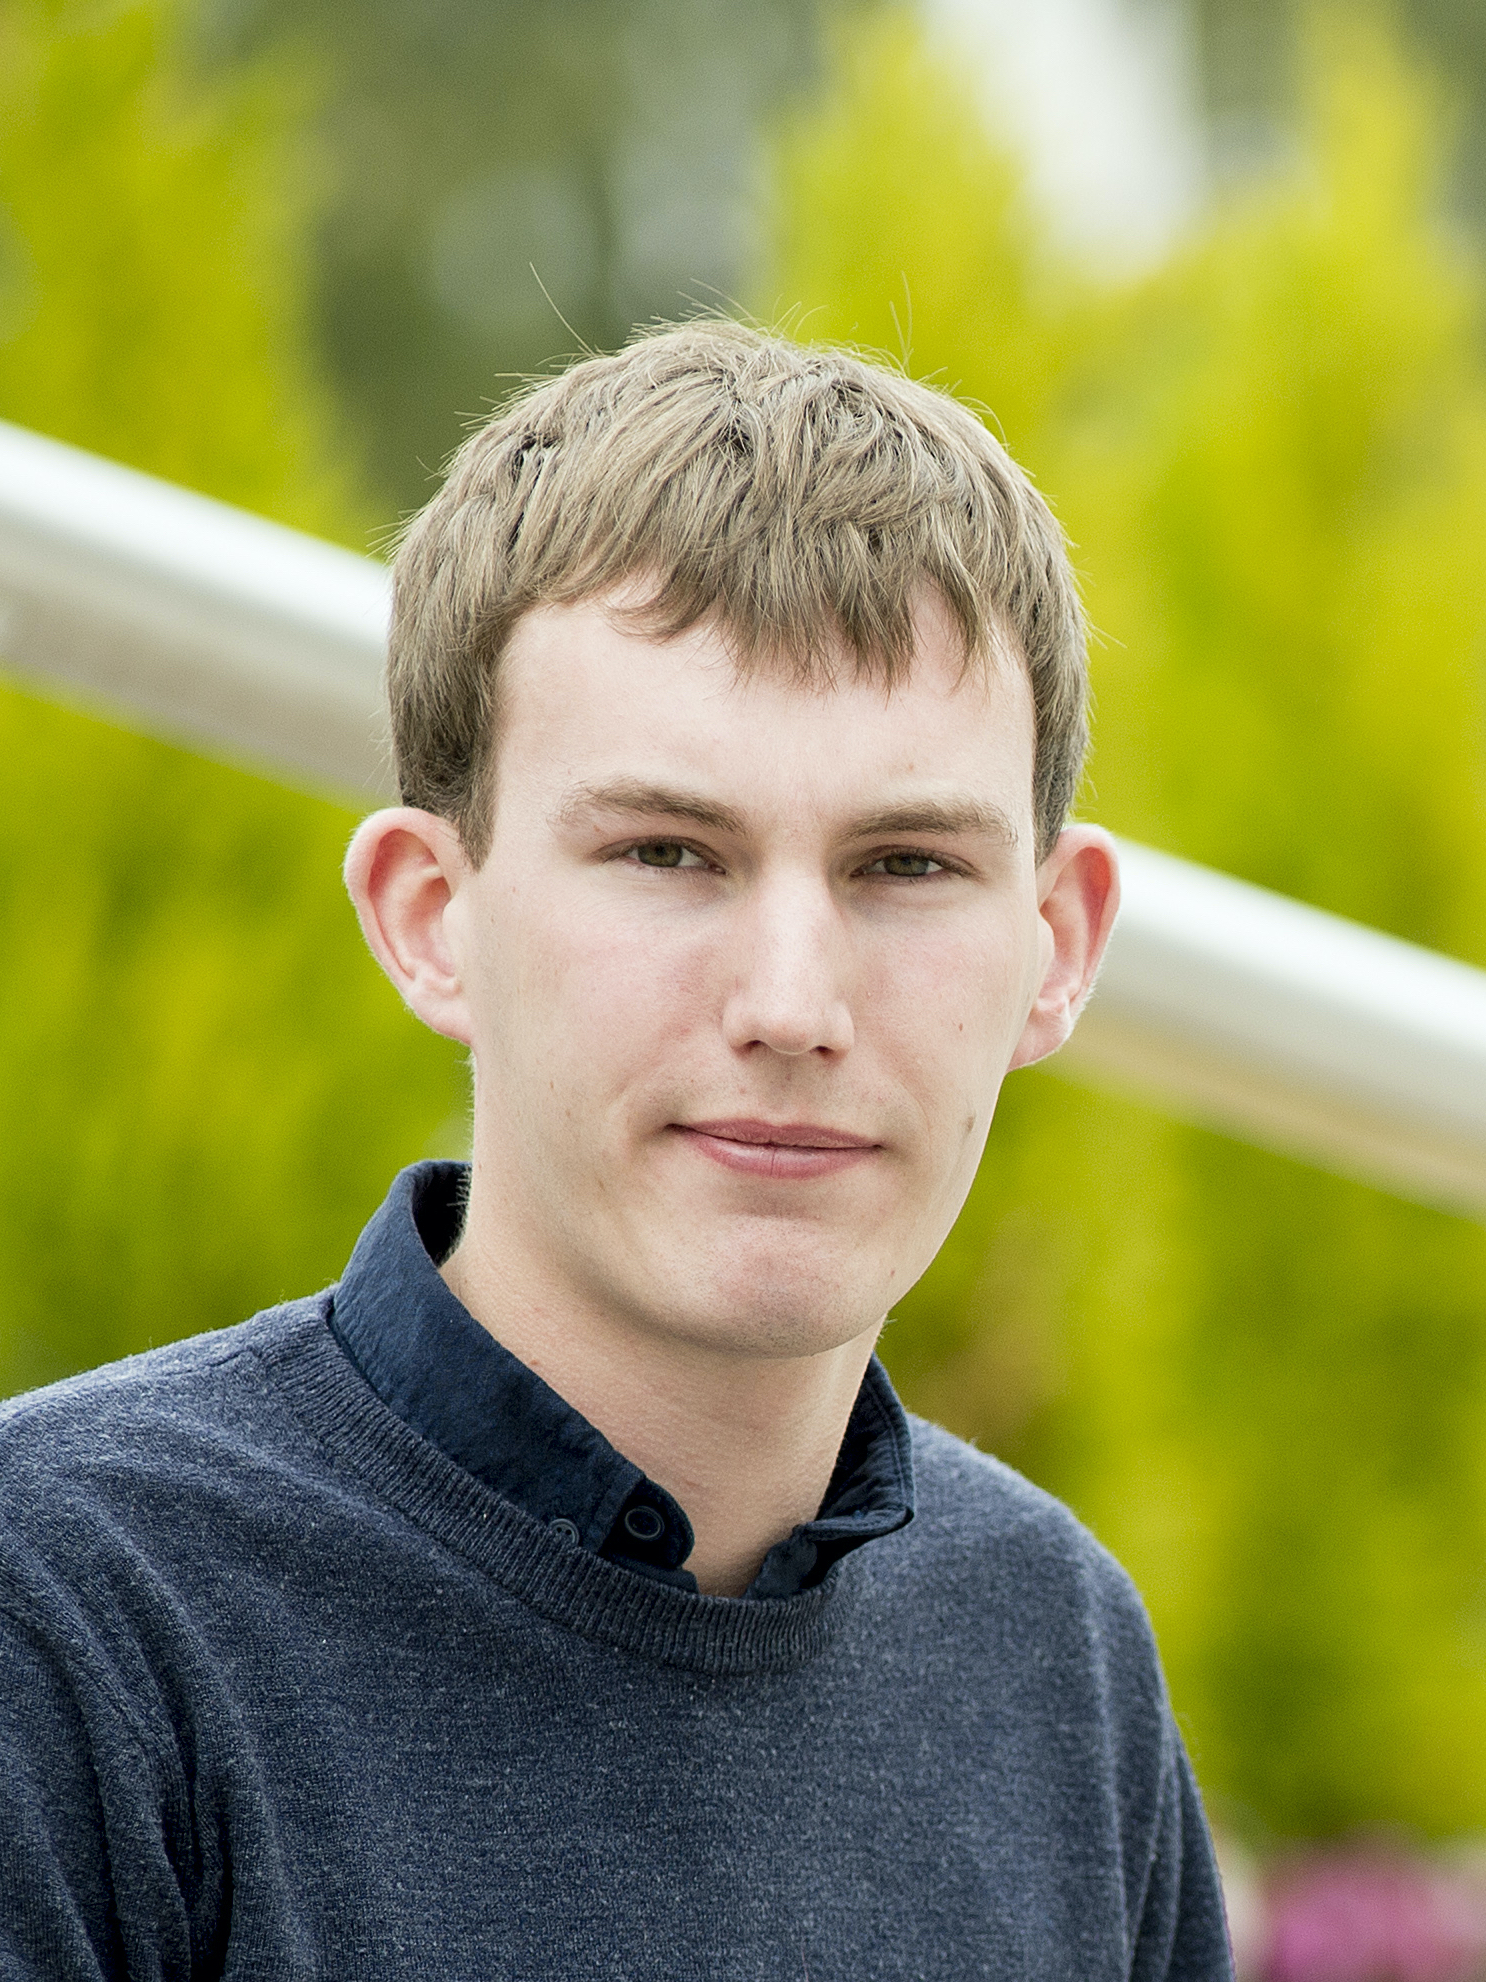
\includegraphics[width=30mm]{dp}\end{flushright}
}

\begin{abstract}
August 2023 edition of SIGLOG Monthly, featuring deadlines, calls and community announcements.
\end{abstract}


\maketitlee

\href{https://lics.siglog.org/newsletters/}{Past Issues}
 - 
\href{https://lics.siglog.org/newsletters/inst.html}{How to submit an announcement}
\section{Table of Content}\begin{itemize}\item DEADLINES (\cref{deadlines}) 
 
\item CALLS 
 
\begin{itemize}\item RSSRail 2023 (CALL FOR PARTICIPATION) (\cref{RSSRail2023})
\item FORMATS 2023 (CALL FOR PARTICIPATION) (\cref{FORMATS2023})
\item Third edition of the UniVr/UniUd Summer School on Formal Methods for Cyber-Physical Systems and Workshop on Synthesis, Monitoring and Learning (CALL FOR PARTICIPATION) (\cref{ThirdeditionoftheUniVrUniUdSummerSchoolonFormalMethodsforCyberPhysicalSystemsandWorkshoponSynthesisMonitoringandLearning})
\item VMCAI 2024 (CALL FOR PAPERS) (\cref{VMCAI2024})
\item OVERLAY 2023 (CALL FOR PAPERS) (\cref{OVERLAY2023})
\item CPP 2024 (CALL FOR PAPERS) (\cref{CPP2024})
\item FLOPS 2024 (CALL FOR PAPERS) (\cref{FLOPS2024})
\item DEON2023 (CALL FOR PAPERS) (\cref{DEON2023})
\end{itemize} 
\item JOB ANNOUNCEMENTS 
 
\begin{itemize}\item PROFESSOR OF COMPUTATIONAL SCIENCE (\cref{PROFESSOROFCOMPUTATIONALSCIENCE})
\end{itemize} 
\end{itemize}\section{Deadlines}\label{deadlines}\rowcolors{1}{white}{gray!25}\begin{tabulary}{\linewidth}{LL}FORMATS 2023:  & Aug 06, 2023 (Early registration deadline) \\
RW 2023:  & Aug 10, 2023 (Application deadline) \\
Infinity 2023:  & Aug 15, 2023 (Talk) \\
UniVr/UniUd:  & Aug 18, 2023 (Applications) \\
PROFESSOR OF COMPUTATIONAL SCIENCE:  & Aug 23, 2023 (Deadline for applications) \\
VMCAI 2024:  & Aug 31, 2023 (Paper) \\
Postoctoral Positions Augusta University (Georgia, USA):  & Sep, 2023 (preferably or until filled) \\
OVERLAY 2023:  & Sep 08, 2023 (Paper) \\
CPP 2024:  & Sep 12, 2023 (Abstract), Sep 19, 2023 (Paper) \\
ICDT 2024:  & Sep 13, 2023 (Cycle 2 Abstract), Sep 20, 2023 (Cycle 2 Full) \\
FLOPS 2024:  & Dec 06, 2023 (Abstract due), Dec 13, 2023 (Papers due) \\
DEON2023:  & Jan 07, 2024 (Paper) \\
\end{tabulary}
\section{RSSRail 2023: International conference on reliability, safety and security of railway systems:  modelling, analysis, verification and certification}\label{RSSRail2023}  October 10-12, 2023 \\ 
  Berlin, Germany \href{https://rssr2023.ebuef.de/}{https://rssr2023.ebuef.de/}\\ 
CALL FOR PARTICIPATION 

\begin{itemize}\item  We would like to invite you to participate in the RSSRail 2023 conference, aiming  to bring together researchers and engineers interested in building critical railway  applications and systems. This will be a working conference in which research  challenges and progress will be discussed and evaluated by both researchers  and engineers, focusing on their potential to be deployed in industrial settings.  
 
  This will be the 5th edition of the RSSRail series with the previous conferences held in Paris, Pistoia, Lille and Paris, again. 
 
  Our plan is to include in the programme three invited talks, technical papers  selected by the PC and four mini-tutorials; see the outline of the programme: \href{https://rssr2023.ebuef.de/program/}{https://rssr2023.ebuef.de/program/} 
 
\item  PROGRAMME 
 
  The programme includes three invited talks (\href{https://rssr2023.ebuef.de/keynotes/}{https://rssr2023.ebuef.de/keynotes/}) 
 
\begin{itemize}\item  Lydia Kaiser, TU Berlin and Einstein Center Digital Future: Unleashing the Potential of Systems Engineering: From Theory to Practice
\item  Andreas Freese, DB Systel: Title to be confirmed.
\item  Aryldo Russo, GESTE ENGINEERING: Continuous Research for Innovation
\end{itemize} 
 The three tutorials are confirmed now, for more information see - \href{https://rssr2023.ebuef.de/tutorials/}{https://rssr2023.ebuef.de/tutorials/} 
 
\begin{itemize}\item SafeRiver,
\item Siemens Mobility \& TÜV Rheinland InterTraffic GmbH, and
\item TU Berlin
\end{itemize} 
 The conference proceedings will be published by Springer in the LNCS series. 
 
\item  REGISTRATION 
 
  \href{https://rssr2023.ebuef.de/registration/}{https://rssr2023.ebuef.de/registration/}  
 
  We are looking forward to welcoming you and your colleagues in Berlin. 
 
\end{itemize}\section{FORMATS 2023: 21st International Conference on Formal Modeling and Analysis of Timed Systems}\label{FORMATS2023}  \href{https://www.uantwerpen.be/en/conferences/confest-2023/formats/}{https://www.uantwerpen.be/en/conferences/confest-2023/formats/}\\ 
  19-21 September 2023, Antwerp, Belgium\\ 
  co-located with CONCUR, FMICS and QEST as part of CONFEST 2023\\ 
CALL FOR PARTICIPATION 

\begin{itemize}\item  FORMATS (International Conference on Formal Modeling and Analysis of Timed Systems) is an annual conference which aims to promote the study of fundamental and practical aspects of timed systems, and to bring together researchers from different disciplines that share interests in the modelling, design and analysis of timed computational systems. 
 
\item  REGISTRATION 
 
  Registration to CONFEST is now open \href{https://www.uantwerpen.be/en/conferences/confest-2023/registration/}{https://www.uantwerpen.be/en/conferences/confest-2023/registration/} 
 
Early registration deadline: Aug 06, 2023 
 
  Note that slightly higher standard prices will apply after August 6th. 
 
\item  INVITED SPEAKERS  
 
  FORMATS 2023 will feature the following invited speakers: 
 
\begin{itemize}\item  Joost-Pieter Katoen, RWTH Aachen University, Germany (joint with all CONFEST conferences)
\item  Nicolas Markey, CNRS \& University of Rennes, France (joint with CONCUR)
\item  David Parker, Oxford University, UK (joint with QEST, CONCUR)
\item  Jaco van de Pol, Aarhus University, Denmark (joint with CONCUR, FMICS)
\end{itemize} 
\item  ACCEPTED PAPERS 
 
  The list of papers that have been accepted for presentation at FORMATS 2023 can be consulted here: 
 
  \href{https://www.uantwerpen.be/en/conferences/confest-2023/formats/papers/}{https://www.uantwerpen.be/en/conferences/confest-2023/formats/papers/} 
 
\end{itemize}\section{Third edition of the UniVr/UniUd Summer School on Formal Methods for Cyber-Physical Systems and Workshop on Synthesis, Monitoring and Learning}\label{ThirdeditionoftheUniVrUniUdSummerSchoolonFormalMethodsforCyberPhysicalSystemsandWorkshoponSynthesisMonitoringandLearning}  UniVr/UniUd:  Udine, August 28-31\\ 
  \href{http://tcs.uniud.it/summer-school}{http://tcs.uniud.it/summer-school} \\ 
  Workshop on Synthesis, Monitoring and Learning - Udine, August 31-September 1\\ 
  \href{http://tcs.uniud.it/smile}{http://tcs.uniud.it/smile}\\ 
CALL FOR PARTICIPATION 

\begin{itemize}\item   Synthesis is a fundamental problem in computer science and mathematics, concerned with automatically generating programs that satisfy a given logical specification. Its applications span a range of domains, including model-based system design, software engineering, and automated theorem proving. For instance, designing a controller that guides the behavior of a reactive system, that is, a system that continually interacts with its environment, can be framed as a synthesis problem. Similarly, the design and verification of a distributed system often depend on distributed synthesis, which finds programs that enforce correct component interaction and satisfy desired specifications. 
 
  The third edition of the Summer School on Formal Methods for Cyber-Physical Systems offers an in-depth exploration of reactive synthesis, a topic that was already introduced in the first edition of the school. The lecturers will provide a systematic account of the main achievements and the current trends of research in reactive synthesis, covering both theory and applications. 
 
  The course will begin with an overview of the classical synthesis problem in the finite-state setting, as originally formulated by Church and solved by Buechi and Landweber. This introductory part will introduce the terminology of infinite two-player games, explain the automatic construction of winning strategies in “regular games”, and address history of the subject, discussing extensions and open problems. From there, the course will investigate approaches for making reactive synthesis more efficient and practical, including techniques for solving the synthesis problem in restricted settings, for decomposing the problem into subproblems, and for employing algorithms, data structures, and heuristics to manage complexity. Variants of the synthesis problem will also be explored, such as control strategies for hybrid and distributed systems, monitor synthesis, synthesis under incomplete information, distributed synthesis, and symmetric synthesis. The implementation of synthesis tools will also receive significant attention, with a focus on recent advances and applications of UPPAAL Stratego and the SYNTCOMP reactive synthesis competition. 
 
  The summer school will conclude with a workshop on emerging research trends in synthesis, monitoring, and learning, which showcases some exciting interactions between formal methods and machine learning. Distinguished invited speakers will lead the workshop. Participants will also have the opportunity to engage with peers from around the world and may propose to deliver short research talks voluntarily. 
 
\item  Lecturers 
 
\begin{itemize}\item  Wolfgang Thomas - RWTH Aachen University, Germany: 3-hour lecture on “Synthesis of strategies in infinite two-player games”
\item  Martin Zimmermann - Aalborg University, Denmark: 3-hour lecture on “Synthesis of infinite-state systems”
\item  Kim G. Larssen - Aalborg University, Denmark: 3-hour lecture on “Synthesis and Optimization for Cyber Physical Systems”
\item  Dana Fisman - Ben Gurion University of the Negev, Israel: 3-hour lecture on “Automata learning of languages of finite and infinite words”
\item  Swen Jacobs - CISPA Helmholtz-Center for Information Security, Germany: 3-hour lecture on “Reactive synthesis: towards practice”
\item  Alessandro Cimatti - Fondazione Bruno Kessler, Italy: 3-hour lecture on “Runtime verification and monitor synthesis”
\end{itemize} 
  See \href{http://tcs.uniud.it/summer-school}{http://tcs.uniud.it/summer-school} for abstracts and programme 
 
\item  Admission and accommodation 
 
  The course is offered in a hybrid format giving the possibility to remotely attend the course (on the Microsoft Teams platform). 
 
  On-site places are limited and assigned on first come first served basis. 
 
  The registration fees are: 
 
\begin{itemize}\item  On-site participation, 250.00 Euro + VAT 22%
\item  Online participation, 120.00 Euro + VAT 22%
\end{itemize} 
  Deadline for online application is August 18, 2023.   
 
  Participation application is available at \href{https://www.cism.it/en/activities/courses/J2303/}{https://www.cism.it/en/activities/courses/J2303/} 
 
\end{itemize}\section{VMCAI 2024: 25th International Conference on Verification, Model Checking, and Abstract Interpretation}\label{VMCAI2024}  January 15-16, 2024, London, United Kingdom\\ 
  \href{https://popl24.sigplan.org/home/VMCAI-2024}{https://popl24.sigplan.org/home/VMCAI-2024}\\ 
CALL FOR PAPERS 

\begin{itemize}\item  VMCAI 2024 is the 25th International Conference on Verification, Model Checking, and Abstract Interpretation. The conference will be held on January 15-16, 2024, in London, UK, co-located with POPL 2024. VMCAI provides a forum for researchers from the communities of Verification, Model Checking, and Abstract Interpretation, facilitating interaction, cross-fertilization, and advancement of hybrid methods that combine these and related areas. 
 
\item  Topics include, but are not limited to: Program Verification; Model Checking; Abstract Interpretation; Abstract Domains; Program Synthesis; Static Analysis; Type Systems; Deductive Methods; Program Logics; First-Order Theories; Decision Procedures; Interpolation; Horn Clause Solving; Program Certification; Separation Logic; Probabilistic Programming and Analysis; Error Diagnosis; Detection of Bugs and Security Vulnerabilities; Program Transformations; Hybrid and Cyber-physical Systems; Concurrent and distributed Systems; Analysis of numerical properties; Analysis of smart contracts; Analysis of neural networks. 
 
\item  All accepted papers will be published in Springer’s Lecture Notes in Computer Science series. Submissions will undergo a single-blind review process. There will be three categories of papers: regular papers, tool papers, and case studies.  
 
\item  Important dates:   
 
\rowcolors{1}{white}{gray!25}\begin{tabulary}{\linewidth}{LL}Paper submission:  & Aug 31, 2023 \\
Notification:  & Oct 11, 2023 \\
Camera-ready:  & Oct 31, 2023 \\
\end{tabulary}
 
\item  Submission details: See \href{https://popl24.sigplan.org/home/VMCAI-2024}{https://popl24.sigplan.org/home/VMCAI-2024} 
 
\end{itemize}\section{OVERLAY 2023}\label{OVERLAY2023}  6th - 9th November, 2023 (the precise day(s) will be announced later)\\ 
  Rome, Italy\\ 
  \href{https://overlay.uniud.it/workshop/2023}{https://overlay.uniud.it/workshop/2023}\\ 
  Co-located with AIxIA 2023\\ 
  \href{http://www.aixia2023.cnr.it/}{http://www.aixia2023.cnr.it/}\\ 
CALL FOR PAPERS 

\begin{itemize}\item   The increasing adoption of Artificial Intelligence techniques in safety-critical systems, employed in real-world scenarios, requires the design of reliable, robust, and verifiable methodologies. Artificial Intelligence systems employed in such applications need to provide formal guarantees about their safety, increasing the need for a close interaction between the Artificial Intelligence and Formal Methods scientific communities, and possibly leading to the proposal of novel neurosymbolic approaches. 
 
  To witness this increasing need, tools and methodologies integrating Formal Methods and Artificial Intelligence, and more broadly symbolic and sub-symbolic solutions, are getting more and more attention, especially considering the wide-range and pervasive applications of machine and deep learning models. 
 
  The workshop is the main official initiative supported by the OVERLAY group (\href{https://overlay.uniud.it}{https://overlay.uniud.it}). The event aims at establishing a stable, long-term scientific forum on relevant topics connected to the relationships between Artificial Intelligence and Formal Methods, by providing a stimulating environment where researchers can discuss opportunities and challenges at the border of the two areas.  
 
  Important goals of the workshop are (i) to encourage the ongoing interaction between the formal methods and artificial intelligence communities, (ii) to identify innovative tools and methodologies, and (iii) to elicit a discussion on open issues and new challenges. 
 
  This year edition will be held between 6th and 9th November 2023 (the precise day(s) will be announced later), as a hybrid workshop co-located with AIxIA 2023 (\href{http://www.aixia2023.cnr.it/}{http://www.aixia2023.cnr.it/}), which is scheduled to be held in Rome, Italy. 
 
  Participants must be registered to AIxIA 2023 (\href{http://www.aixia2023.cnr.it/}{http://www.aixia2023.cnr.it/}). Overlay does not have an additional specific fee. 
 
\item  Invited speaker  
 
  Luciano Serafini - Fondazione Bruno Kessler, Italy 
 
\item  Call for contributions   
 
  We accept extended abstracts (4 pages + references) focusing on the interaction between Artificial Intelligence and Formal Methods and on the issue of symbolic/sub-symbolic integration. Invited talks will complement the presentations of contributed papers. 
 
  Topics of interest include (but are not limited to): automata theory; automated reasoning; automated planning and scheduling; controller synthesis; formal specification languages; formal verification; game theory; hybrid and discrete systems; logics in computer science; neurosymbolic approaches; logic for neural networks; neural networks for logic; reactive synthesis; runtime verification and monitoring; satisfiability modulo theories and theorem proving; specification and verification of machine/deep learning systems; tools and applications 
 
  Contributed papers can present recent results at the border of the two fields, new research directions, challenges and perspectives. Presentation of results recently published in other scientific journals or conferences is also welcome. 
 
  We plan to include all papers in the Proceedings of the event, published at CEUR Workshop Proceedings. CEUR WS proceedings are archival proceedings indexed by DBLP and Scopus. 
 
  Submitted papers should not exceed four (4) pages plus references. Authors are asked to use CEUR's LaTeX style, available at \href{https://overlay.uniud.it/workshop/2023/CEURART.zip}{https://overlay.uniud.it/workshop/2023/CEURART.zip}.  
 
  Submissions must be in PDF format and will be handled via the EasyChair Conference system at the following address: \href{https://easychair.org/my/conference?conf=overlay2023}{https://easychair.org/my/conference?conf=overlay2023}. 
 
\item  Important dates 
 
\rowcolors{1}{white}{gray!25}\begin{tabulary}{\linewidth}{LL}Paper submission:  & Sep 08, 2023 \\
Acceptance notification:  & Sep 22, 2023 \\
Camera-ready submission:  & Oct 15, 2023 \\
Workshop:  & between Nov 6-9, 2023 (the precise day(s) will be announced later) \\
\end{tabulary}
 
\end{itemize}\section{CPP 2024: Certified Proofs and Programs}\label{CPP2024}  15-16 January 2024, London, UK (co-located with POPL 2024)\\ 
  \href{https://popl24.sigplan.org/home/CPP-2024}{https://popl24.sigplan.org/home/CPP-2024}\\ 
CALL FOR PAPERS 

  Certified Programs and Proofs (CPP) is an international conference on practical and theoretical topics in all areas that consider formal verification and certification as an essential paradigm for their work. CPP spans areas of computer science, mathematics, logic, and education.\\ 
\begin{itemize}\item  IMPORTANT DATES 
 
\rowcolors{1}{white}{gray!25}\begin{tabulary}{\linewidth}{LL}Abstract submission:  & Sep 12, 2023 \\
Paper submission:  & Sep 19, 2023 \\
Notification (tentative):  & Nov 21, 2023 \\
Camera Ready Deadline (tentative):  & Mid December 2023 (TBA) \\
Conference:  & 15-16 January 2024 \\
\end{tabulary}
 
  Deadlines expire at the end of the day, anywhere on earth. Abstract and submission deadlines are strict and there will be no extensions. The full call for papers is available at: \href{https://popl24.sigplan.org/home/CPP-2024#Call-for-Papers}{https://popl24.sigplan.org/home/CPP-2024\#Call-for-Papers} 
 
\end{itemize}\section{FLOPS 2024: 17th International Symposium on Functional and Logic Programming}\label{FLOPS2024}  May 15-17, 2024, Kumamoto, Japan\\ 
  \href{https://conf.researchr.org/home/flops-2024}{https://conf.researchr.org/home/flops-2024}\\ 
CALL FOR PAPERS 

\begin{itemize}\item  FLOPS aims to bring together practitioners, researchers and implementers of declarative programming, to discuss mutually interesting results and common problems: theoretical advances, their implementations in language systems and tools, and applications of these systems in practice. The scope includes all aspects of the design, semantics, theory, applications, implementations, and teaching of declarative programming. FLOPS specifically aims to promote cross-fertilization between theory and practice and among different styles of declarative programming. 
 
\item  FLOPS solicits original papers in all areas of declarative programming: 
 
\begin{itemize}\item  functional, logic, functional-logic programming, rewriting systems, formal methods, and model checking, program transformations, and program refinements, developing programs with the help of theorem provers or SAT/SMT solvers, verifying properties of programs using declarative programming techniques;
\item  foundations, language design, implementation issues (compilation techniques, memory management, run-time systems, etc.),     applications, and case studies.
\end{itemize} 
\item  SUBMISSIONS 
 
\begin{itemize}\item  Regular research papers: they should describe new results and will be judged on originality, correctness, and significance.
\item  System descriptions: they should describe a working system and will be judged on originality, usefulness, and design.
\item  Declarative pearls: new and excellent declarative programs or theories with illustrative applications.
\end{itemize} 
\item  DATES (AoE) 
 
\rowcolors{1}{white}{gray!25}\begin{tabulary}{\linewidth}{LL}Abstract due:  & Dec 06, 2023 \\
Papers due:  & Dec 13, 2023 \\
Notifications:  & Jan 31, 2024 \\
Final versions due:  & Feb 28, 2024 \\
\end{tabulary}
 
\end{itemize}\section{DEON2023: SPECIAL ISSUE ON DEONTIC LOGIC AND NORMATIVE SYSTEMS}\label{DEON2023}  Journal of Applied Logics – IfCoLog Journal (open access)\\ 
  \href{http://www.uqtr.ca/DEON2023/Special.Issue}{http://www.uqtr.ca/DEON2023/Special.Issue}\\ 
CALL FOR PAPERS 

\begin{itemize}\item  The special issue will focus on the theme Theoretical and technical limitations of automated behavior. 
 
\item  Important dates: 
 
Paper submission: Jan 07, 2024 
 
\item  Guest editors: Clayton Peterson (Université du Québec à Trois-Rivières) and Christian Strasser (Ruhr-Universität Bochum) 
 
\item  Detailed information can be found on the webpage. 
 
\end{itemize}\section{PROFESSOR OF COMPUTATIONAL SCIENCE}\label{PROFESSOROFCOMPUTATIONALSCIENCE}  CALL FOR APPLICATIONS\\ 
JOB ANNOUNCEMENT 

\begin{itemize}\item  Peter Paule will retire end of September 2023. As a consequence, the Johannes Kepler University Linz is announcing the position of a PROFESSOR OF COMPUTATIONAL SCIENCE assigned to the Research Institute for Symbolic Computation (RISC) and to begin as soon as possible. 
 
Deadline for applications: Aug 23, 2023 
 
  For further details of the application (in particular, the job profile) see \href{https://www.jku.at/en/work-at-the-jku/job-openings/professorship-positions/professor-of-computational-science/}{https://www.jku.at/en/work-at-the-jku/job-openings/professorship-positions/professor-of-computational-science/} 
 
  In case of questions concerning the position, do not hesitate to contact Carsten Schneider Carsten.Schneider@risc.jku.at.  
 
\end{itemize}


\bigskip Links: \href{http://siglog.org/}{SIGLOG website}, \href{https://lics.siglog.org}{LICS website}, \href{https://lics.siglog.org/newsletters/}{SIGLOG Monthly}\end{document}